% Nallino, Part II p. 256: the arc of visibility, redrawn from the print at the size of the print. The coordinates are
% those of a 400 dpi render of the figure (crop from x 108 pt, y 530 pt of the master page; y downward). BA is the
% horizon, DEG the ecliptic, ZBD the vertical circle through the centre D of the Sun; E, H and T are points of the
% horizon, HK and TL (dashed) the perpendiculars on the ecliptic.
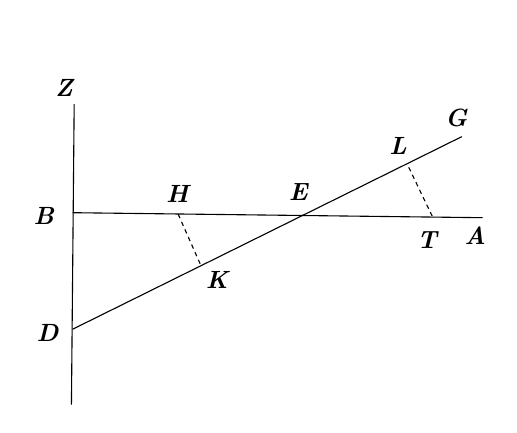
\begin{tikzpicture}[x=0.0635mm,y=-0.0635mm,line width=0.4pt,every node/.style={font=\bfseries\itshape\small,inner sep=1pt}]
\path (60,-37);
\draw (153,116) -- (147.5,717);
\draw (150,333) -- (970,343);
\draw (150,566) -- (928,181);
\draw[dash pattern=on 1.6pt off 1.4pt] (361,336) -- (407,440);
\draw[dash pattern=on 1.6pt off 1.4pt] (869,340) -- (820,238);
\node at (132.5,83) {Z};
\node at (917,143) {G};
\node at (800.5,199) {L};
\node at (359,296.5) {H};
\node at (601,292.5) {E};
\node at (92,340.5) {B};
\node at (858.5,388) {T};
\node at (955,380.5) {A};
\node at (438.5,467) {K};
\node at (99.5,573.5) {D};
\end{tikzpicture}
